\paragraph{Note:}
The following text and accompanying architectural diagram (Fig.\ \ref{fig:archiver-arch}) provide a high-level overview of my chat archiving utility.
For brevity, I focus on the system's design and core functionality rather than technical specifics.
Complete source code and additional materials are available in dedicated repositories.

The main repository of the archiving utility, \emph{chat-archiver}%
\footnote{\repoRef{chat-archiver}{chat-archiver}}%
, contains the core system implementation. A separate repository for the chat conversion and Markdown \enquote{rendering} functionality%
\footnote{\repoRef{chat-renderer}{chat-renderer}}
is included as a git submodule \cite{git-submodules}.

The database container configuration is located in my \emph{project} repository%
\footnote{\repoRef{project}{project}}%
, which contains various resources accumulated during this thesis with broader relevance across different project components.
Since I also used the database for generic code optimization testing, I moved its container configuration to this shared repository during development.

Backups of the database are archived in the \emph{project-db-dump} repository%
\footnote{\repoRef{project-db-dump}{project-db-dump}}%
, and Markdown-converted chat logs are available in the \emph{chats} repository%
\footnote{\repoRef{chats}{chats}}.


\begin{figure}[h]
  \centering
  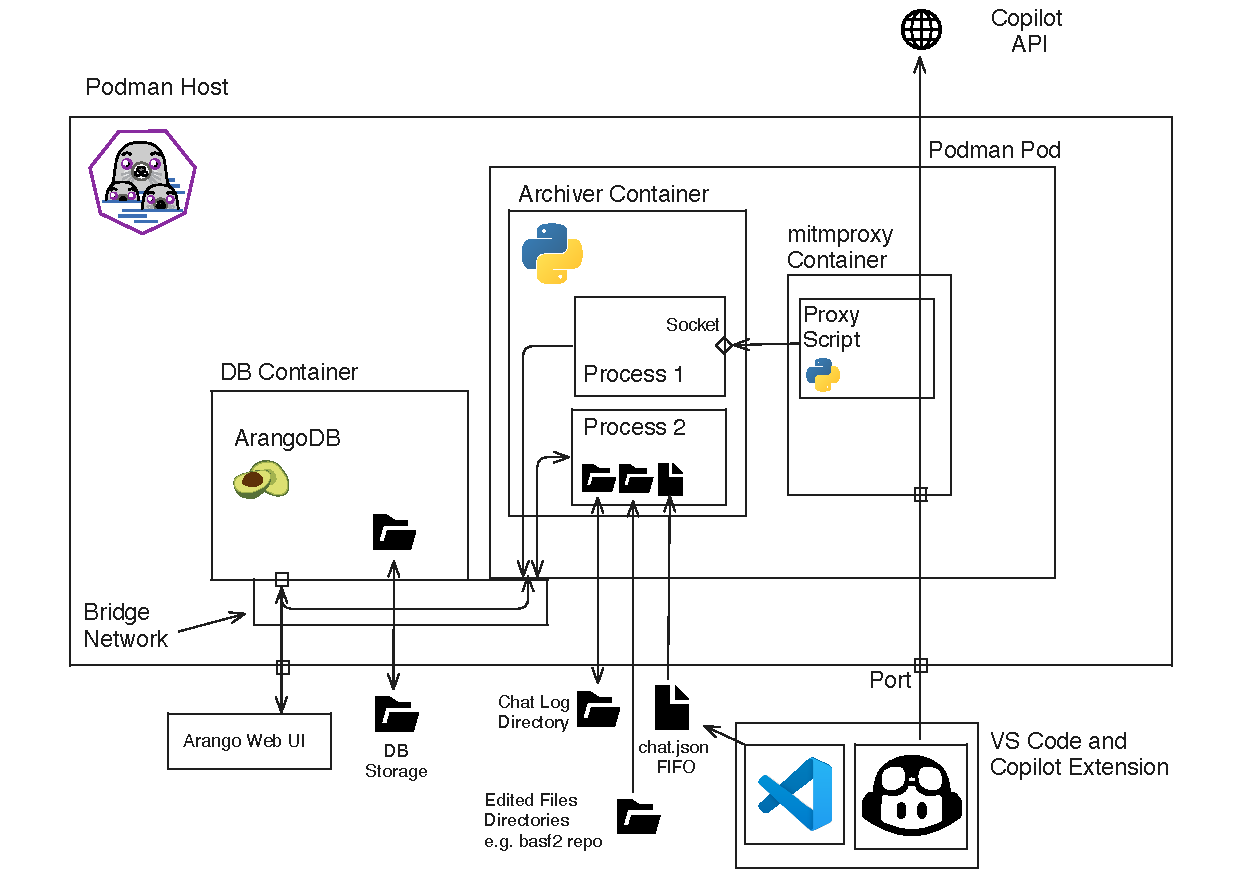
\includegraphics[width=\textwidth]{static/diagram.pdf}
  \caption{Architecture Diagram of the Chat Archiver\footnotemark}
  \label{fig:archiver-arch}
\end{figure}%
\footnotetext{
  Icon Sources:
  \cite{svg-1}%
  \cite{svg-2}%
  \cite{svg-3}%
  \cite{svg-4}%
  \cite{svg-5}%
  \cite{svg-6}%
  \cite{svg-7}%
  \cite{svg-8}%
  \cite{svg-9}%
}


To support my work, I developed a chat archiver designed to back up and convert chat logs exported from the GitHub Copilot extension in Visual Studio Code. The goal was to transform raw JSON chat data into a human-readable, annotated Markdown format.
Each chat entry is enriched with metadata, including the specific model used to generate the response, the runtime of each request, and file diffs for any edits performed by Copilot.

However, the exported JSON logs do not include model information by default.
To recover this missing data, I implemented a more involved solution that intercepts the network traffic of the Copilot extension.
This is achieved by routing all VS Code traffic through mitmproxy \cite{mitmproxy} (Man-In-The-Middle proxy).

This software allows to extract and process relevant data from the network stream with custom Python scripts that filter HTTP(S) requests passing through the proxy.
I configured such a script to intercept only requests to Copilot API endpoints.

The entire system runs inside a containerized environment using Podman \cite{podman}. 
Within a Podman pod, mitmproxy operates in one container, while a second container runs the Python-based archiving script.
In Podman, a pod is a facility that groups containers, allowing them for example to share the same network namespace.

The archiving script executes two core processes:
\begin{enumerate}[topsep=0pt]
  \item \textbf{Listener Process}: This process receives relevant intercepted Copilot API data via a network socket, specifically the LLM identifier that generated a chat response along with the associated internal message ID.
  The mitmproxy Python user-script transmits this information after extracting it from HTTP requests to Copilot's chat completion API endpoint.

  \item \textbf{Archiver Process}: This second process reads data from a named pipe (FIFO) mounted into the container from the host system. When a JSON chat log is exported from VS Code and written to the FIFO, the process first saves the raw JSON document to the database. It then parses the chat data and converts it into a Markdown file.
\end{enumerate}

The JSON chat logs include the internal Copilot message IDs, which allows the archiver to associate responses with their corresponding models by querying the database of previously stored model--ID pairs. 

Additionally, the utility generates diffs for any file edits made during conversations in Copilot's Agent or Edit modes.
For diff generation to work, edited files must be accessible from within the container. 
To ensure this, I mounted the necessary directories into the container in read-only mode, namely the basf2 directory during V0Fitter refactoring, and the directory containing the task files for generic code optimization testing.

The generated Markdown files are saved to a mounted output directory, allowing direct access from the host system.

For all database needs throughout the thesis, I used ArangoDB \cite{arangodb}.
A key advantage of ArangoDB over traditional SQL databases is its document database functionality, which allows direct storage of JSON-like documents and flexible querying of their keys and values.
This was particularly beneficial for storing and analyzing the chat log JSON documents and intercepted API responses.

I used ArangoDB not only for chat archiving purposes but also for storing benchmarking data related to the generic code optimization tests. 
The database therefore runs in a separate container outside the archiving pod, with persistent storage mounted from the host. 
To enable communication between the database container and the archiver pod, they are connected via a shared bridge network \cite{bridge-network}.